
\documentclass{article}\usepackage[]{graphicx}\usepackage[]{color}
% maxwidth is the original width if it is less than linewidth
% otherwise use linewidth (to make sure the graphics do not exceed the margin)
\makeatletter
\def\maxwidth{ %
  \ifdim\Gin@nat@width>\linewidth
    \linewidth
  \else
    \Gin@nat@width
  \fi
}
\makeatother

\definecolor{fgcolor}{rgb}{0.345, 0.345, 0.345}
\newcommand{\hlnum}[1]{\textcolor[rgb]{0.686,0.059,0.569}{#1}}%
\newcommand{\hlstr}[1]{\textcolor[rgb]{0.192,0.494,0.8}{#1}}%
\newcommand{\hlcom}[1]{\textcolor[rgb]{0.678,0.584,0.686}{\textit{#1}}}%
\newcommand{\hlopt}[1]{\textcolor[rgb]{0,0,0}{#1}}%
\newcommand{\hlstd}[1]{\textcolor[rgb]{0.345,0.345,0.345}{#1}}%
\newcommand{\hlkwa}[1]{\textcolor[rgb]{0.161,0.373,0.58}{\textbf{#1}}}%
\newcommand{\hlkwb}[1]{\textcolor[rgb]{0.69,0.353,0.396}{#1}}%
\newcommand{\hlkwc}[1]{\textcolor[rgb]{0.333,0.667,0.333}{#1}}%
\newcommand{\hlkwd}[1]{\textcolor[rgb]{0.737,0.353,0.396}{\textbf{#1}}}%
\let\hlipl\hlkwb

\usepackage{framed}
\makeatletter
\newenvironment{kframe}{%
 \def\at@end@of@kframe{}%
 \ifinner\ifhmode%
  \def\at@end@of@kframe{\end{minipage}}%
  \begin{minipage}{\columnwidth}%
 \fi\fi%
 \def\FrameCommand##1{\hskip\@totalleftmargin \hskip-\fboxsep
 \colorbox{shadecolor}{##1}\hskip-\fboxsep
     % There is no \\@totalrightmargin, so:
     \hskip-\linewidth \hskip-\@totalleftmargin \hskip\columnwidth}%
 \MakeFramed {\advance\hsize-\width
   \@totalleftmargin\z@ \linewidth\hsize
   \@setminipage}}%
 {\par\unskip\endMakeFramed%
 \at@end@of@kframe}
\makeatother

\definecolor{shadecolor}{rgb}{.97, .97, .97}
\definecolor{messagecolor}{rgb}{0, 0, 0}
\definecolor{warningcolor}{rgb}{1, 0, 1}
\definecolor{errorcolor}{rgb}{1, 0, 0}
\newenvironment{knitrout}{}{} % an empty environment to be redefined in TeX

\usepackage{alltt}


\usepackage{amsmath}
\usepackage{amscd}
\usepackage[tableposition=top]{caption}
\usepackage{ifthen}
\usepackage[utf8]{inputenc}



\IfFileExists{upquote.sty}{\usepackage{upquote}}{}
\begin{document}

Load necessary libraries:
\begin{knitrout}
\definecolor{shadecolor}{rgb}{0.969, 0.969, 0.969}\color{fgcolor}\begin{kframe}
\begin{alltt}
\hlkwd{library}\hlstd{(ggplot2)}
\hlkwd{library}\hlstd{(ggvis)}
\end{alltt}


{\ttfamily\noindent\itshape\color{messagecolor}{\#\# \\\#\# Attaching package: 'ggvis'}}

{\ttfamily\noindent\itshape\color{messagecolor}{\#\# The following object is masked from 'package:ggplot2':\\\#\# \\\#\#\ \ \ \  resolution}}\begin{alltt}
\hlkwd{library}\hlstd{(dplyr)}
\end{alltt}


{\ttfamily\noindent\itshape\color{messagecolor}{\#\# \\\#\# Attaching package: 'dplyr'}}

{\ttfamily\noindent\itshape\color{messagecolor}{\#\# The following objects are masked from 'package:stats':\\\#\# \\\#\#\ \ \ \  filter, lag}}

{\ttfamily\noindent\itshape\color{messagecolor}{\#\# The following objects are masked from 'package:base':\\\#\# \\\#\#\ \ \ \  intersect, setdiff, setequal, union}}\begin{alltt}
\hlkwd{library}\hlstd{(RColorBrewer)}
\end{alltt}
\end{kframe}
\end{knitrout}

Function of $H_{adm}$ in terms of $H_1,H_2,\gamma_1$, and $F_{12}$:
\begin{knitrout}
\definecolor{shadecolor}{rgb}{0.969, 0.969, 0.969}\color{fgcolor}\begin{kframe}
\begin{alltt}
\hlstd{Hadm} \hlkwb{<-} \hlkwa{function}\hlstd{(}\hlkwc{H1}\hlstd{,} \hlkwc{H2}\hlstd{,} \hlkwc{gamma1}\hlstd{,} \hlkwc{F12}\hlstd{)}
\hlstd{\{}
  \hlstd{gamma1}\hlopt{^}\hlnum{2}\hlopt{*}\hlstd{H1}\hlopt{+}\hlstd{(}\hlnum{1}\hlopt{-}\hlstd{gamma1)}\hlopt{^}\hlnum{2}\hlopt{*}\hlstd{H2}\hlopt{+}
    \hlstd{gamma1}\hlopt{*}\hlstd{(}\hlnum{1}\hlopt{-}\hlstd{gamma1)}\hlopt{*}\hlstd{(H1}\hlopt{+}\hlstd{H2)}\hlopt{*}\hlstd{(}\hlnum{1}\hlopt{+}\hlstd{F12)}\hlopt{/}\hlstd{(}\hlnum{1}\hlopt{-}\hlstd{F12)}
\hlstd{\}}
\end{alltt}
\end{kframe}
\end{knitrout}

Get some realistic values of $H_1$ and $H_2$ as means of expected heterozygosities for the European and Native American populations in the Pemberton et al 2013 \textit{G3} paper:
\begin{knitrout}
\definecolor{shadecolor}{rgb}{0.969, 0.969, 0.969}\color{fgcolor}\begin{kframe}
\begin{alltt}
\hlstd{HetsEuro} \hlkwb{<-} \hlkwd{c}\hlstd{(}\hlnum{0.724}\hlstd{,}\hlnum{0.728}\hlstd{,}\hlnum{0.731}\hlstd{,}\hlnum{0.718}\hlstd{,}\hlnum{0.730}\hlstd{,}\hlnum{0.727}\hlstd{,}\hlnum{0.723}\hlstd{,}\hlnum{0.735}\hlstd{)}
\hlkwd{length}\hlstd{(HetsEuro)}
\end{alltt}
\begin{verbatim}
## [1] 8
\end{verbatim}
\begin{alltt}
\hlstd{H1} \hlkwb{<-} \hlkwd{mean}\hlstd{(HetsEuro)}

\hlstd{HetsNAm} \hlkwb{<-} \hlkwd{c}\hlstd{(}\hlnum{0.625}\hlstd{,}\hlnum{0.561}\hlstd{,}\hlnum{0.507}\hlstd{,}\hlnum{0.676}\hlstd{,}\hlnum{0.617}\hlstd{,}
             \hlnum{0.671}\hlstd{,}\hlnum{0.695}\hlstd{,}\hlnum{0.696}\hlstd{,}\hlnum{0.665}\hlstd{,}\hlnum{0.644}\hlstd{,}
             \hlnum{0.641}\hlstd{,}\hlnum{0.665}\hlstd{,}\hlnum{0.582}\hlstd{,}\hlnum{0.623}\hlstd{,}\hlnum{0.660}\hlstd{,}
             \hlnum{0.667}\hlstd{,}\hlnum{0.649}\hlstd{,}\hlnum{0.483}\hlstd{,}\hlnum{0.624}\hlstd{,}\hlnum{0.669}\hlstd{,}
             \hlnum{0.580}\hlstd{,}
             \hlnum{0.643}\hlstd{,}\hlnum{0.640}\hlstd{,}\hlnum{0.671}\hlstd{,}\hlnum{0.590}\hlstd{,}\hlnum{0.587}\hlstd{,}
             \hlnum{0.625}\hlstd{,}\hlnum{0.625}\hlstd{,}\hlnum{0.633}\hlstd{)}
\hlkwd{length}\hlstd{(HetsNAm)}
\end{alltt}
\begin{verbatim}
## [1] 29
\end{verbatim}
\begin{alltt}
\hlstd{H2} \hlkwb{<-} \hlkwd{mean}\hlstd{(HetsNAm)}

\hlstd{H1}
\end{alltt}
\begin{verbatim}
## [1] 0.727
\end{verbatim}
\begin{alltt}
\hlstd{H2}
\end{alltt}
\begin{verbatim}
## [1] 0.628069
\end{verbatim}
\end{kframe}
\end{knitrout}

Get the region where $\underline{\gamma_{\max}}=\gamma^*$ in terms of $H_1$ and $H_2$:
\begin{knitrout}
\definecolor{shadecolor}{rgb}{0.969, 0.969, 0.969}\color{fgcolor}\begin{kframe}
\begin{alltt}
\hlkwd{abs}\hlstd{(H1}\hlopt{-}\hlstd{H2)}\hlopt{/}\hlstd{(}\hlnum{2}\hlopt{*}\hlstd{(H1}\hlopt{+}\hlstd{H2)}\hlopt{+}\hlkwd{abs}\hlstd{(H1}\hlopt{-}\hlstd{H2))}
\end{alltt}
\begin{verbatim}
## [1] 0.03521844
\end{verbatim}
\end{kframe}
\end{knitrout}

Get values of $H_{adm}$ for $\gamma_1 \in [0,1]$ and various values of $F_{12}$:
\begin{knitrout}
\definecolor{shadecolor}{rgb}{0.969, 0.969, 0.969}\color{fgcolor}\begin{kframe}
\begin{alltt}
\hlstd{minFst} \hlkwb{<-} \hlstd{(}\hlnum{2}\hlopt{-}\hlstd{H1}\hlopt{-}\hlstd{H2}\hlopt{-}\hlnum{2}\hlopt{*}\hlkwd{sqrt}\hlstd{((}\hlnum{1}\hlopt{-}\hlstd{H1)}\hlopt{*}\hlstd{(}\hlnum{1}\hlopt{-}\hlstd{H2)))}\hlopt{/}
  \hlstd{(}\hlnum{2}\hlopt{+}\hlstd{H1}\hlopt{+}\hlstd{H2}\hlopt{-}\hlnum{2}\hlopt{*}\hlkwd{sqrt}\hlstd{((}\hlnum{1}\hlopt{-}\hlstd{H1)}\hlopt{*}\hlstd{(}\hlnum{1}\hlopt{-}\hlstd{H2)))}
\hlstd{maxFst} \hlkwb{<-} \hlstd{(}\hlnum{2}\hlopt{-}\hlstd{H1}\hlopt{-}\hlstd{H2)}\hlopt{/}\hlstd{(}\hlnum{2}\hlopt{+}\hlstd{H1}\hlopt{+}\hlstd{H2)}
\hlstd{FstGammaStr} \hlkwb{<-} \hlkwd{abs}\hlstd{(H1}\hlopt{-}\hlstd{H2)}\hlopt{/}\hlstd{(}\hlnum{2}\hlopt{*}\hlstd{(H1}\hlopt{+}\hlstd{H2}\hlopt{+}\hlkwd{abs}\hlstd{(H1}\hlopt{-}\hlstd{H2)))}

\hlstd{HadmDF} \hlkwb{<-} \hlkwd{expand.grid}\hlstd{(}\hlkwc{gamma1}\hlstd{=}\hlkwd{seq}\hlstd{(}\hlnum{0}\hlstd{,}\hlnum{1}\hlstd{,}\hlkwc{by} \hlstd{=} \hlnum{0.01}\hlstd{),}
                      \hlkwc{Fst}\hlstd{=}\hlkwd{c}\hlstd{(minFst,}\hlnum{0.02}\hlstd{,FstGammaStr,}\hlnum{0.06}\hlstd{,}\hlnum{0.10}\hlstd{,}
                            \hlnum{0.14}\hlstd{,}\hlnum{0.18}\hlstd{,maxFst))}
\hlstd{HadmDF}\hlopt{$}\hlstd{Hadm} \hlkwb{<-} \hlnum{NA}
\hlkwa{for}\hlstd{(i} \hlkwa{in} \hlnum{1}\hlopt{:}\hlkwd{nrow}\hlstd{(HadmDF))}
\hlstd{\{}
  \hlstd{HadmDF}\hlopt{$}\hlstd{Hadm[i]} \hlkwb{<-} \hlkwd{Hadm}\hlstd{(}\hlkwc{H1} \hlstd{= H1,} \hlkwc{H2} \hlstd{= H2,}
                         \hlkwc{gamma1} \hlstd{= HadmDF}\hlopt{$}\hlstd{gamma1[i],}
                         \hlkwc{F12} \hlstd{= HadmDF}\hlopt{$}\hlstd{Fst[i])}
\hlstd{\}}

\hlstd{HadmDF}\hlopt{$}\hlstd{Fst} \hlkwb{<-} \hlkwd{round}\hlstd{(HadmDF}\hlopt{$}\hlstd{Fst,} \hlnum{3}\hlstd{)}
\end{alltt}
\end{kframe}
\end{knitrout}

Make a 2nd data frame with just the boundary for the region where the maximum of $H_{adm}$ is at $\gamma^*$:
\begin{knitrout}
\definecolor{shadecolor}{rgb}{0.969, 0.969, 0.969}\color{fgcolor}\begin{kframe}
\begin{alltt}
\hlstd{HadmDFB1} \hlkwb{<-} \hlstd{HadmDF[HadmDF}\hlopt{$}\hlstd{Fst} \hlopt{==} \hlnum{0.034}\hlstd{,]}
\hlstd{HadmDFB2} \hlkwb{<-} \hlstd{HadmDF[HadmDF}\hlopt{$}\hlstd{Fst} \hlopt{==} \hlnum{0.192}\hlstd{,]}
\hlkwd{identical}\hlstd{(HadmDFB1[,}\hlnum{1}\hlstd{], HadmDFB2[,}\hlnum{1}\hlstd{])}
\end{alltt}
\begin{verbatim}
## [1] TRUE
\end{verbatim}
\begin{alltt}
\hlstd{HadmDF2} \hlkwb{<-} \hlkwd{data.frame}\hlstd{(}\hlkwc{gamma1} \hlstd{= HadmDFB1}\hlopt{$}\hlstd{gamma1,}
                      \hlkwc{HadmB1} \hlstd{= HadmDFB1}\hlopt{$}\hlstd{Hadm,}
                      \hlkwc{HadmB2} \hlstd{= HadmDFB2}\hlopt{$}\hlstd{Hadm)}
\end{alltt}
\end{kframe}
\end{knitrout}

Add some more things to data frame to work with ggplot:
\begin{knitrout}
\definecolor{shadecolor}{rgb}{0.969, 0.969, 0.969}\color{fgcolor}\begin{kframe}
\begin{alltt}
\hlstd{HadmDF}\hlopt{$}\hlstd{Fst} \hlkwb{<-} \hlkwd{as.factor}\hlstd{(HadmDF}\hlopt{$}\hlstd{Fst)}

\hlstd{HadmDF} \hlkwb{<-} \hlstd{HadmDF} \hlopt
  \hlkwd{group_by}\hlstd{(Fst)} \hlopt
  \hlkwd{mutate}\hlstd{(}\hlkwc{HadmMax} \hlstd{= (}\hlkwd{max}\hlstd{(Hadm)} \hlopt{==} \hlstd{Hadm))}
\end{alltt}
\end{kframe}
\end{knitrout}

Specify colors:
\begin{knitrout}
\definecolor{shadecolor}{rgb}{0.969, 0.969, 0.969}\color{fgcolor}\begin{kframe}
\begin{alltt}
\hlcom{##the default colors are just equally spaced colors on the color wheel}
\hlcom{##from: http://stackoverflow.com/questions/8197559/emulate-ggplot2-default-color-palette}
\hlstd{gg_color_hue} \hlkwb{<-} \hlkwa{function}\hlstd{(}\hlkwc{n}\hlstd{) \{}
  \hlstd{hues} \hlkwb{=} \hlkwd{seq}\hlstd{(}\hlnum{15}\hlstd{,} \hlnum{375}\hlstd{,} \hlkwc{length}\hlstd{=n}\hlopt{+}\hlnum{1}\hlstd{)}
  \hlkwd{hcl}\hlstd{(}\hlkwc{h}\hlstd{=hues,} \hlkwc{l}\hlstd{=}\hlnum{65}\hlstd{,} \hlkwc{c}\hlstd{=}\hlnum{100}\hlstd{)[}\hlnum{1}\hlopt{:}\hlstd{n]}
\hlstd{\}}

\hlstd{grey} \hlkwb{<-} \hlkwd{grey.colors}\hlstd{(}\hlnum{7}\hlstd{)[}\hlnum{3}\hlstd{]}

\hlcom{##ggCols5 <- gg_color_hue(5)}
\hlstd{ggCols5} \hlkwb{<-} \hlkwd{brewer.pal}\hlstd{(}\hlnum{7}\hlstd{,} \hlstr{"BuPu"}\hlstd{)[}\hlopt{-}\hlstd{(}\hlnum{1}\hlopt{:}\hlnum{2}\hlstd{)]}
\end{alltt}
\end{kframe}
\end{knitrout}

Get the values of Hadm over all values of gamma1, Fst in a tight grid:
\begin{knitrout}
\definecolor{shadecolor}{rgb}{0.969, 0.969, 0.969}\color{fgcolor}\begin{kframe}
\begin{alltt}
\hlstd{Hadm_all_allow} \hlkwb{<-}
  \hlkwd{expand.grid}\hlstd{(}\hlkwc{gamma1}\hlstd{=}\hlkwd{seq}\hlstd{(}\hlnum{0}\hlstd{,}\hlnum{1}\hlstd{,}\hlkwc{by} \hlstd{=} \hlnum{0.005}\hlstd{),}
              \hlkwc{Fst}\hlstd{=}\hlkwd{seq}\hlstd{(minFst,maxFst,}\hlkwc{length.out}\hlstd{=}\hlnum{200}\hlstd{))}
\hlstd{Hadm_all_allow}\hlopt{$}\hlstd{Hadm} \hlkwb{<-} \hlnum{NA}
\hlkwa{for}\hlstd{(i} \hlkwa{in} \hlnum{1}\hlopt{:}\hlkwd{nrow}\hlstd{(Hadm_all_allow))}
\hlstd{\{}
  \hlstd{Hadm_all_allow}\hlopt{$}\hlstd{Hadm[i]} \hlkwb{<-}
    \hlkwd{Hadm}\hlstd{(}\hlkwc{H1} \hlstd{= H1,} \hlkwc{H2} \hlstd{= H2,}
         \hlkwc{gamma1} \hlstd{= Hadm_all_allow}\hlopt{$}\hlstd{gamma1[i],}
         \hlkwc{F12} \hlstd{= Hadm_all_allow}\hlopt{$}\hlstd{Fst[i])}
\hlstd{\}}
\hlkwd{head}\hlstd{(Hadm_all_allow)}
\end{alltt}
\begin{verbatim}
##   gamma1         Fst      Hadm
## 1  0.000 0.002808579 0.6280690
## 2  0.005 0.002808579 0.6286016
## 3  0.010 0.002808579 0.6291338
## 4  0.015 0.002808579 0.6296657
## 5  0.020 0.002808579 0.6301972
## 6  0.025 0.002808579 0.6307283
\end{verbatim}
\begin{alltt}
\hlkwd{tail}\hlstd{(Hadm_all_allow)}
\end{alltt}
\begin{verbatim}
##       gamma1       Fst      Hadm
## 40195  0.975 0.1922259 0.7402469
## 40196  0.980 0.1922259 0.7376620
## 40197  0.985 0.1922259 0.7350449
## 40198  0.990 0.1922259 0.7323955
## 40199  0.995 0.1922259 0.7297139
## 40200  1.000 0.1922259 0.7270000
\end{verbatim}
\begin{alltt}
\hlcom{##now for each value of Fst, get the maximum value}
\hlstd{Hadm_max} \hlkwb{<-} \hlkwd{data.frame}\hlstd{(}\hlkwc{Fst}\hlstd{=}\hlkwd{seq}\hlstd{(minFst,maxFst,}\hlkwc{length.out}\hlstd{=}\hlnum{200}\hlstd{),}
                       \hlkwc{gamma1_argmax}\hlstd{=}\hlnum{NA}\hlstd{,}
                       \hlkwc{Hadm_max}\hlstd{=}\hlnum{NA}\hlstd{)}
\hlkwa{for}\hlstd{(i} \hlkwa{in} \hlnum{1}\hlopt{:}\hlkwd{nrow}\hlstd{(Hadm_max))}
\hlstd{\{}
  \hlcom{##get all rows of Hadm_all_allow with this value of Fst}
  \hlstd{current_Fst} \hlkwb{<-} \hlstd{Hadm_max}\hlopt{$}\hlstd{Fst[i]}
  \hlstd{subset_Fst} \hlkwb{<-}
    \hlstd{Hadm_all_allow[Hadm_all_allow}\hlopt{$}\hlstd{Fst} \hlopt{==} \hlstd{current_Fst,]}
  \hlcom{##get argmax and max}
  \hlstd{current_argmax} \hlkwb{<-} \hlkwd{which.max}\hlstd{(subset_Fst}\hlopt{$}\hlstd{Hadm)}
  \hlstd{Hadm_max}\hlopt{$}\hlstd{gamma1_argmax[i]} \hlkwb{<-} \hlstd{subset_Fst}\hlopt{$}\hlstd{gamma1[current_argmax]}
  \hlstd{Hadm_max}\hlopt{$}\hlstd{Hadm_max[i]} \hlkwb{<-} \hlstd{subset_Fst}\hlopt{$}\hlstd{Hadm[current_argmax]}
\hlstd{\}}
\end{alltt}
\end{kframe}
\end{knitrout}

Make some plots:
\begin{knitrout}
\definecolor{shadecolor}{rgb}{0.969, 0.969, 0.969}\color{fgcolor}\begin{kframe}
\begin{alltt}
\hlkwd{head}\hlstd{(HadmDF}\hlopt{$}\hlstd{Fst)}
\end{alltt}
\begin{verbatim}
## [1] 0.003 0.003 0.003 0.003 0.003 0.003
## Levels: 0.003 0.02 0.034 0.06 0.1 0.14 0.18 0.192
\end{verbatim}
\begin{alltt}
\hlcom{##rewrite this as a function of gamma1 primarily}
\hlstd{Hadm} \hlkwb{<-} \hlkwa{function}\hlstd{(}\hlkwc{gamma1}\hlstd{,} \hlkwc{H1}\hlstd{,} \hlkwc{H2}\hlstd{,} \hlkwc{F12}\hlstd{)}
\hlstd{\{}
  \hlstd{gamma1}\hlopt{^}\hlnum{2}\hlopt{*}\hlstd{H1}\hlopt{+}\hlstd{(}\hlnum{1}\hlopt{-}\hlstd{gamma1)}\hlopt{^}\hlnum{2}\hlopt{*}\hlstd{H2}\hlopt{+}
    \hlstd{gamma1}\hlopt{*}\hlstd{(}\hlnum{1}\hlopt{-}\hlstd{gamma1)}\hlopt{*}\hlstd{(H1}\hlopt{+}\hlstd{H2)}\hlopt{*}\hlstd{(}\hlnum{1}\hlopt{+}\hlstd{F12)}\hlopt{/}\hlstd{(}\hlnum{1}\hlopt{-}\hlstd{F12)}
\hlstd{\}}

\hlstd{HadmDF}\hlopt{$}\hlstd{Fst} \hlkwb{<-} \hlkwd{factor}\hlstd{(HadmDF}\hlopt{$}\hlstd{Fst,} \hlkwc{levels}\hlstd{=}\hlkwd{rev}\hlstd{(}\hlkwd{levels}\hlstd{(HadmDF}\hlopt{$}\hlstd{Fst)))}

\hlkwd{ggplot}\hlstd{(HadmDF)} \hlopt{+}
  \hlkwd{geom_ribbon}\hlstd{(}\hlkwc{data}\hlstd{=HadmDF2,} \hlkwd{aes}\hlstd{(}\hlkwc{x}\hlstd{=gamma1,} \hlkwc{ymin}\hlstd{=HadmB1,} \hlkwc{ymax}\hlstd{=HadmB2),}
              \hlkwc{fill}\hlstd{=}\hlstr{"grey"}\hlstd{,} \hlkwc{alpha}\hlstd{=}\hlnum{0.4}\hlstd{)} \hlopt{+}
  \hlkwd{geom_line}\hlstd{(}\hlkwd{aes}\hlstd{(}\hlkwc{x}\hlstd{=gamma1,} \hlkwc{y}\hlstd{=Hadm,} \hlkwc{group}\hlstd{=Fst,} \hlkwc{col}\hlstd{=Fst,}
                \hlkwc{lty}\hlstd{=Fst),} \hlkwc{size}\hlstd{=}\hlnum{1.2}\hlstd{)} \hlopt{+}
  \hlkwd{geom_point}\hlstd{(}\hlkwd{aes}\hlstd{(}\hlkwc{x}\hlstd{=gamma1,} \hlkwc{y}\hlstd{=Hadm,} \hlkwc{size}\hlstd{=HadmMax))} \hlopt{+}
  \hlkwd{geom_hline}\hlstd{(}\hlkwc{yintercept}\hlstd{=}\hlkwd{c}\hlstd{(H1,H2),} \hlkwc{size}\hlstd{=}\hlnum{1.2}\hlstd{)} \hlopt{+}
  \hlkwd{geom_line}\hlstd{(}\hlkwc{data}\hlstd{=Hadm_max,}
            \hlkwd{aes}\hlstd{(}\hlkwc{x}\hlstd{=gamma1_argmax,} \hlkwc{y}\hlstd{=Hadm_max),}
            \hlkwc{color}\hlstd{=}\hlstr{"red"}\hlstd{,} \hlkwc{size}\hlstd{=}\hlnum{1.2}\hlstd{)} \hlopt{+}
  \hlkwd{ylim}\hlstd{(}\hlkwd{c}\hlstd{(}\hlnum{0.45}\hlstd{,}\hlnum{0.9}\hlstd{))} \hlopt{+}
  \hlkwd{scale_color_manual}\hlstd{(}\hlkwc{values}\hlstd{=}\hlkwd{c}\hlstd{(grey, ggCols5[}\hlnum{1}\hlopt{:}\hlnum{4}\hlstd{],}
                              \hlstr{"#000000"}\hlstd{,}
                              \hlstd{ggCols5[}\hlnum{5}\hlstd{], grey),}
                     \hlkwd{guide_legend}\hlstd{(}\hlkwc{title}\hlstd{=}\hlkwd{quote}\hlstd{(Fst)),}
                     \hlkwc{labels} \hlstd{=} \hlkwd{c}\hlstd{(}\hlstr{"0.192"}\hlstd{,}\hlstr{"0.18"}\hlstd{,}\hlstr{"0.14"}\hlstd{,}\hlstr{"0.10"}\hlstd{,}
                                \hlstr{"0.06"}\hlstd{,}\hlstr{"0.034"}\hlstd{,}\hlstr{"0.02"}\hlstd{,}\hlstr{"0.003"}\hlstd{))} \hlopt{+}
  \hlkwd{scale_size_manual}\hlstd{(}\hlkwc{values} \hlstd{=} \hlkwd{c}\hlstd{(}\hlnum{NA}\hlstd{,} \hlnum{2.5}\hlstd{))} \hlopt{+}
  \hlkwd{scale_linetype_manual}\hlstd{(}\hlkwc{values} \hlstd{=} \hlkwd{c}\hlstd{(}\hlnum{1}\hlstd{,}\hlnum{3}\hlstd{,}\hlnum{2}\hlstd{,}\hlnum{4}\hlstd{,}\hlnum{5}\hlstd{,}\hlnum{1}\hlstd{,}\hlnum{6}\hlstd{,}\hlnum{1}\hlstd{),}
                        \hlkwd{guide_legend}\hlstd{(}\hlkwc{title}\hlstd{=}\hlkwd{quote}\hlstd{(Fst)),}
                        \hlkwc{labels} \hlstd{=} \hlkwd{c}\hlstd{(}\hlstr{"0.192"}\hlstd{,}\hlstr{"0.18"}\hlstd{,}\hlstr{"0.14"}\hlstd{,}\hlstr{"0.10"}\hlstd{,}
                                   \hlstr{"0.06"}\hlstd{,}\hlstr{"0.034"}\hlstd{,}\hlstr{"0.02"}\hlstd{,}\hlstr{"0.003"}\hlstd{))} \hlopt{+}
  \hlkwd{theme}\hlstd{(}\hlkwc{axis.line} \hlstd{=} \hlkwd{element_line}\hlstd{(}\hlkwc{colour} \hlstd{=} \hlstr{"black"}\hlstd{),}
        \hlkwc{plot.title} \hlstd{=} \hlkwd{element_text}\hlstd{(}\hlkwc{size} \hlstd{=} \hlnum{16}\hlstd{,} \hlkwc{hjust} \hlstd{=} \hlnum{0.5}\hlstd{),}
        \hlkwc{panel.grid.major} \hlstd{=} \hlkwd{element_blank}\hlstd{(),}
        \hlkwc{panel.grid.minor} \hlstd{=} \hlkwd{element_blank}\hlstd{(),}
        \hlkwc{panel.border} \hlstd{=} \hlkwd{element_blank}\hlstd{(),}
        \hlkwc{panel.background} \hlstd{=} \hlkwd{element_blank}\hlstd{(),}
        \hlkwc{legend.key} \hlstd{=} \hlkwd{element_blank}\hlstd{(),}
        \hlkwc{legend.text.align} \hlstd{=} \hlnum{0}\hlstd{,}
        \hlkwc{text} \hlstd{=} \hlkwd{element_text}\hlstd{(}\hlkwc{size}\hlstd{=}\hlnum{20}\hlstd{),}
        \hlkwc{axis.title.x} \hlstd{=} \hlkwd{element_text}\hlstd{(}\hlkwc{size}\hlstd{=}\hlnum{20}\hlstd{),}
        \hlkwc{axis.title.y} \hlstd{=} \hlkwd{element_text}\hlstd{(}\hlkwc{size}\hlstd{=}\hlnum{20}\hlstd{),}
        \hlkwc{axis.text.x} \hlstd{=} \hlkwd{element_text}\hlstd{(}\hlkwc{size}\hlstd{=}\hlnum{14}\hlstd{),}
        \hlkwc{axis.text.y} \hlstd{=} \hlkwd{element_text}\hlstd{(}\hlkwc{size}\hlstd{=}\hlnum{14}\hlstd{))} \hlopt{+}
  \hlkwd{ylab}\hlstd{(}\hlkwd{expression}\hlstd{(H[adm]))} \hlopt{+}
  \hlcom{##xlab(expression(gamma[1])) +}
  \hlkwd{xlab}\hlstd{(}\hlkwd{expression}\hlstd{(}\hlkwd{atop}\hlstd{(gamma[}\hlnum{1}\hlstd{],} \hlstr{"Ancestry in population 1"}\hlstd{)))} \hlopt{+}
  \hlkwd{guides}\hlstd{(}\hlkwc{size}\hlstd{=}\hlnum{FALSE}\hlstd{,}
         \hlkwc{color}\hlstd{=}\hlkwd{guide_legend}\hlstd{(}\hlkwc{title}\hlstd{=}\hlkwd{expression}\hlstd{(F[st])),}
         \hlkwc{linetype}\hlstd{=}\hlkwd{guide_legend}\hlstd{(}\hlkwc{title}\hlstd{=}\hlkwd{expression}\hlstd{(F[st])))}
\end{alltt}


{\ttfamily\noindent\color{warningcolor}{\#\# Warning: Removed 800 rows containing missing values (geom\_point).}}\end{kframe}
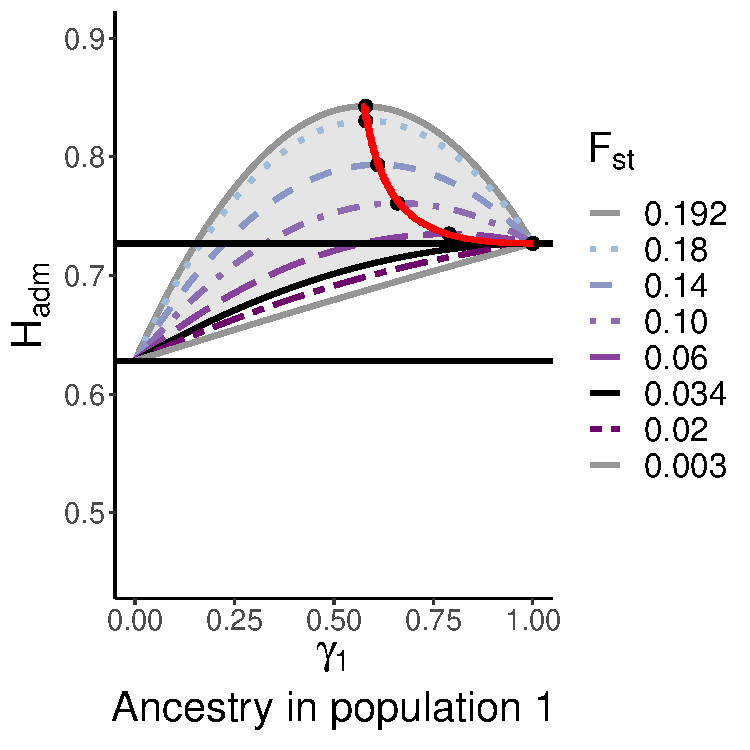
\includegraphics[width=\maxwidth]{../figs/Fig1-1} 

\end{knitrout}

\end{document}
